\section{Drone racing: definition and implications}

As in any race, competitors measure their skills at maneuvering their vehicle,
from within or at distance, against the clock or against themselves, in an
attempt to complete a circuit before everyone else.

In drone racing, the circuit consists of a set of obstacles, static or
dynamic, usually arranged in a loop. For the case of classic drone racing, huge
futuristic-looking arenas are used as a playground for extremely skilled pilots,
who make the race look impressive and dynamic by the use of FPV goggles to fly
the drones at very high speed, reaching 120mph~\cite{DRL}.

\begin{figure}[h]
	\centering
	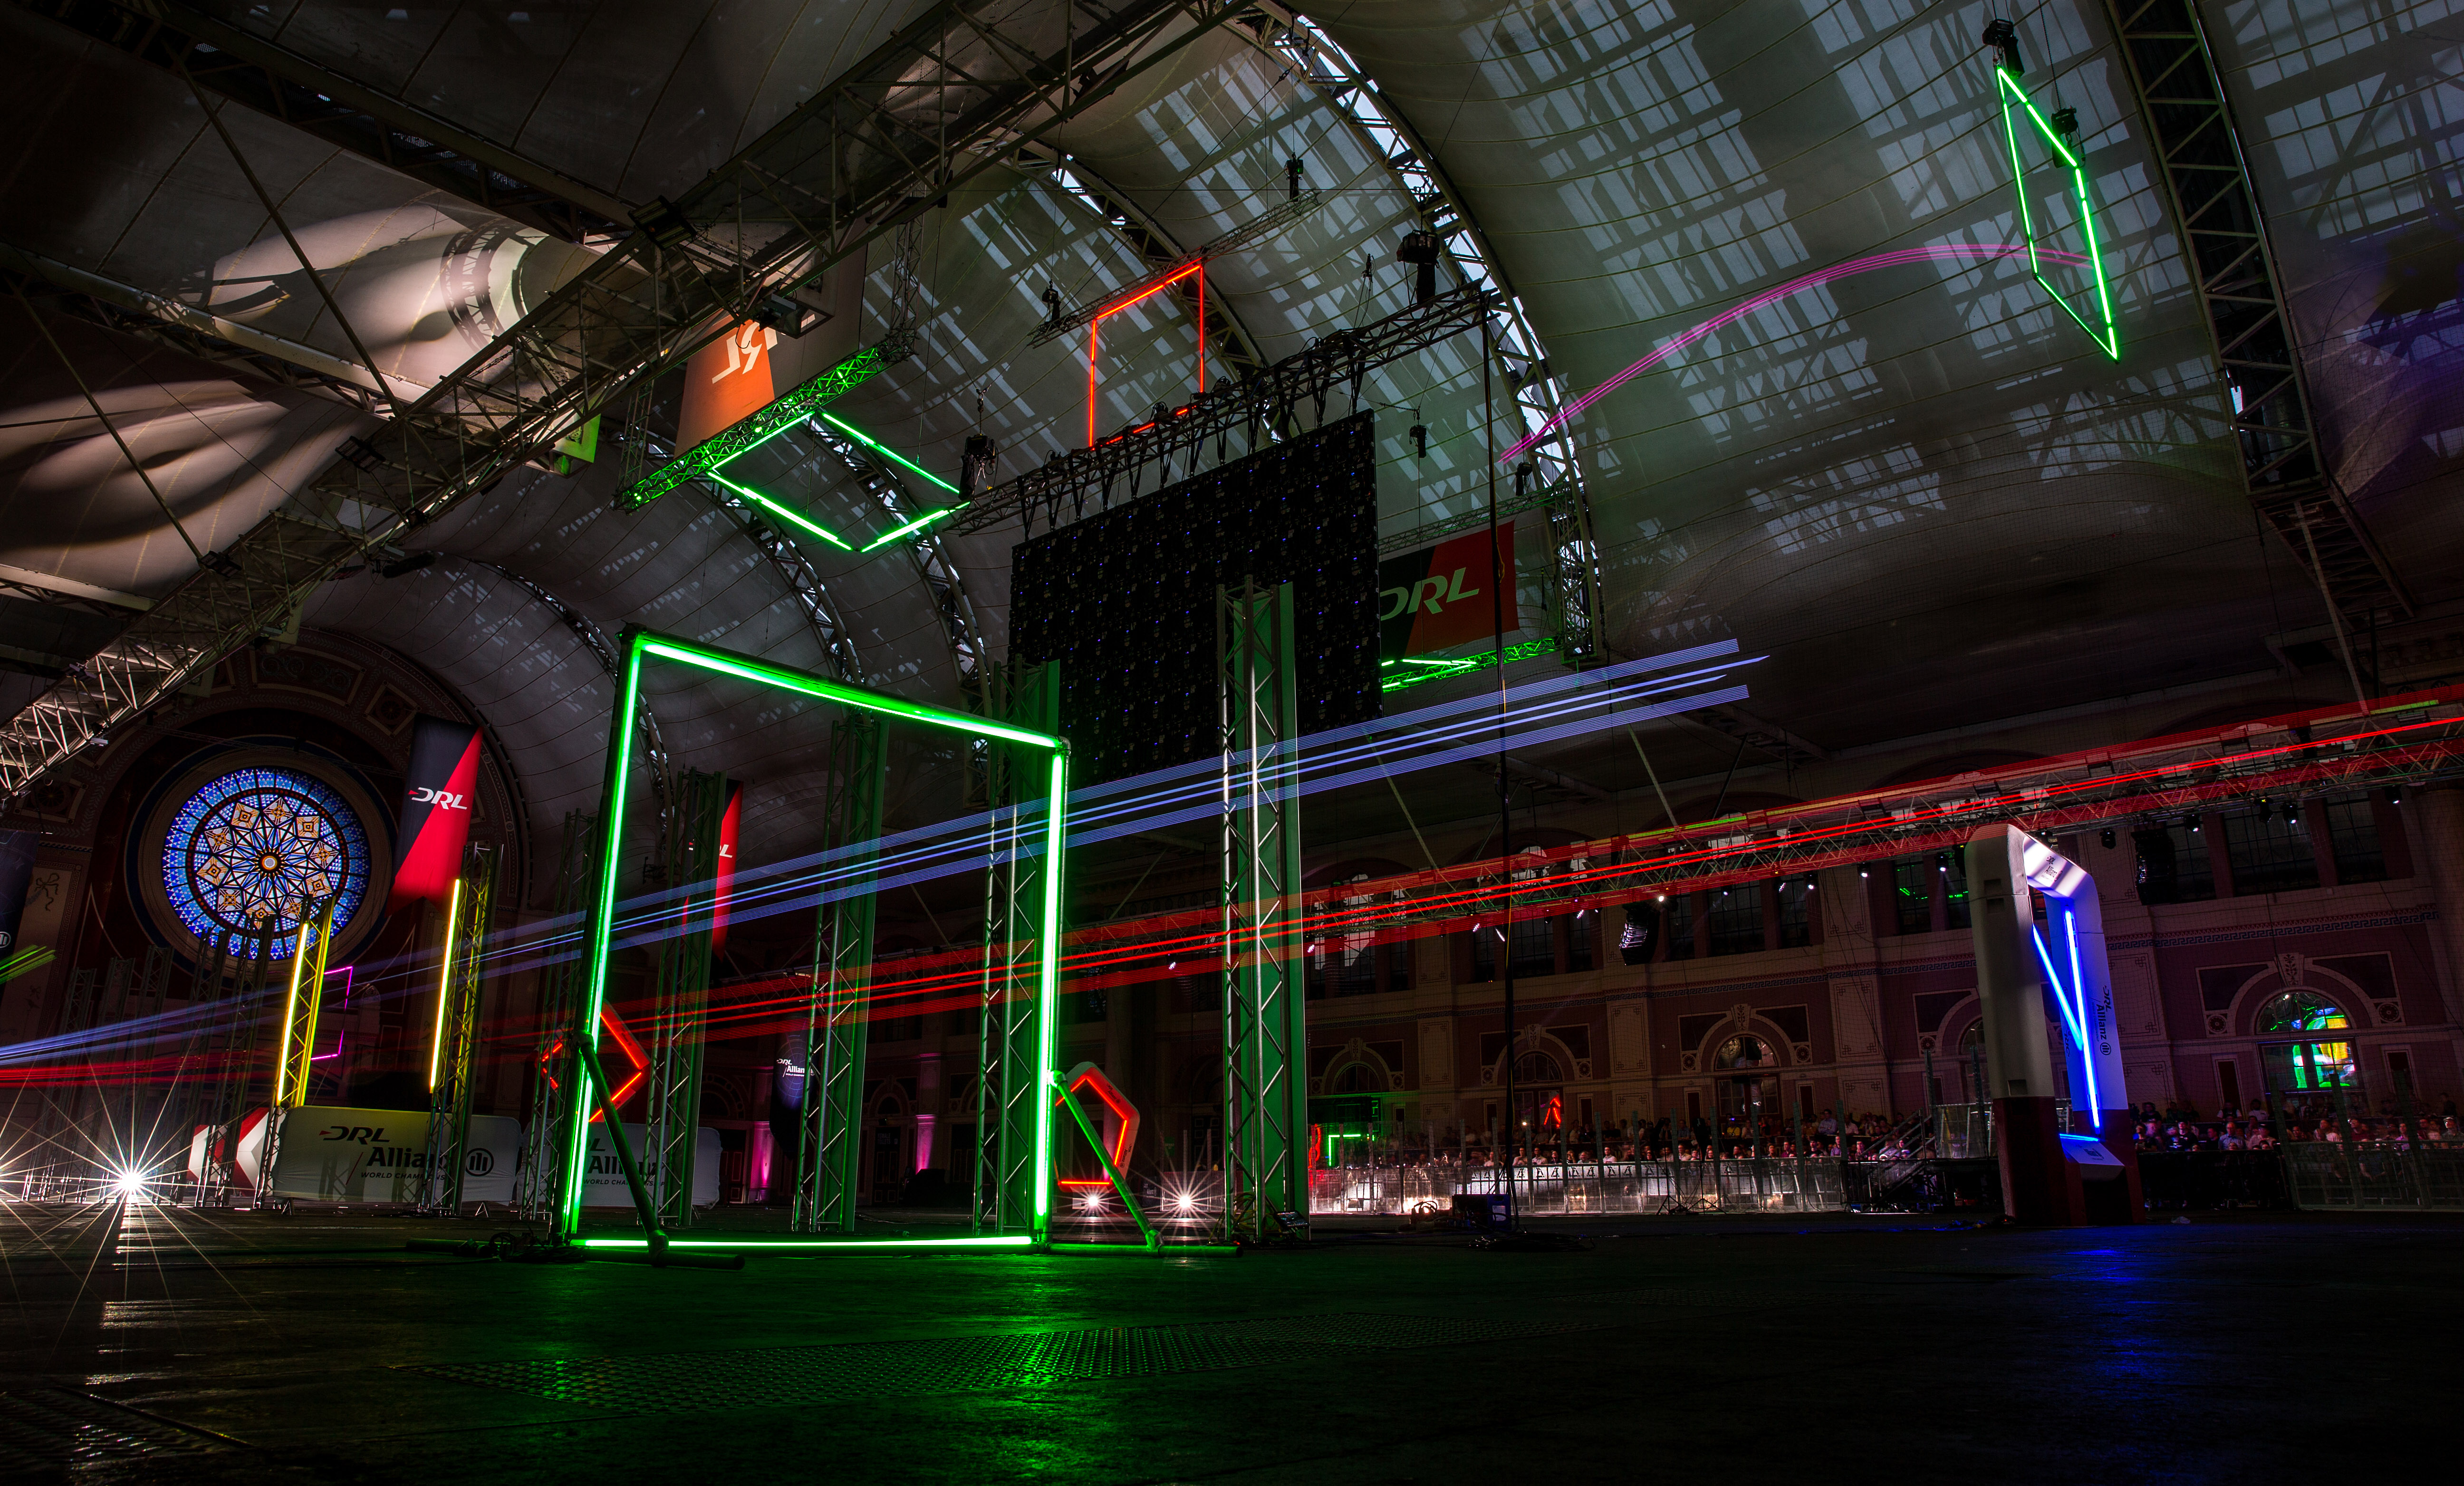
\includegraphics[width=0.5\textwidth]{figure/drl_arena.jpg}
	\caption{Drone Racing League arena in London (Steven
	Paston/PA)~\cite{DRLRecord}}
\end{figure}

For the case of autonomous drone racing, up until the \emph{Drone Racing
League} announced their autonomous competition of 2019, arenas looked much more
like a laboratory than a glowing circuit, as it can be seen in
Fig.~\ref{fig:mygates} showing the AiR Lab in Skejby (Aarhus, DK), with its
gates built and painted for this work. These obstacles were inspired by the
previous competitions organized by IROS, as seen in Fig.~\ref{fig:iros} which
also shows the typical type of drones used in this research area: consumer
drones for the larger audience. This kind of drones is not made for sportive
flight, but mostly for an easy hands-on experience, providing a relatively slow
but stable flight.

The goal is to complete a given amount of turns as fast as possible, but since
it is still the early days of drone racing and the costs of a potential crash
would be too high, each drone races against the clock, one after another.
Ultimately, autonomous drones will be racing against skilled pilots, as the
\emph{Drone Racing League} seems to encourage it by giving a total prize of two
million USD for the race of 2019~\cite{LockheedDRL}.


\subsubsection{Challenges}

What makes drone racing such an interesting challenge to work on for autonomous
UAVs, is the cumulative complexity of each sub-problem to be solved, namely:

\begin{itemize}
	\item{\textbf{Obstacle detection\\}
		The very first challenge to be solved is the detection of the obstacles
		on the circuit, whose shape and color can vary from competition to
		competition, and can even have dynamic properties with moving parts to
		avoid. This rather computer vision-centric problem can be solved
		in many ways, but a compromise has to be made between accuracy and
		robustness/adaptability.
	}
	\item{\textbf{Collision avoidance\\}
		In the simplest case of autonomous drone racing, the circuit is often
		composed of thin obstacles to be crossed (as seen in
		Fig.~\ref{fig:mygates}), which means that the trajectory of the drone
		has little chance of encountering obstacles to avoid, if calculated
		accurately. However, it would be a valuable asset for the UAV to have
		some sort of collision avoidance system, in the case where the planned
		trajectory is wrong and the drone would crash into an obstacle, for
		instance.
	}
	\item{\textbf{Path planning\\}
		Without doubts, the most important task for an autonomous drone in the
		case of a race, is to plan its trajectory in accordance with its
		surroundings. An efficient trajectory must be as direct as possible,
		from point A to B, where B is usually a gate through which the drone
		has to pass, or even the end point of the race (in which case the
		trajectory must also go through every gate).
	}
	\item{\textbf{Circuit compliance\\}
		Being able to generate an efficient trajectory is already an
		achievement, but it is to no use in a race if it is not respecting the
		order of the obstacles which the drone must fly through. In some cases,
		a rough map of the circuit is given a short time before the
		competition, so that participants can take the desired trajectory into
		consideration when developing their algorithm.
	}
	\item{\textbf{Aggressive flight\\}
		Last but not least, any pilot, being human or software, must be able to
		drive fast and aggressively in order to have a chance of winning a
		race.  Nevertheless, this is a challenge on its own that does not need
		to be solved until every building block of the auto-pilot system is
		robust and efficient.\\
	}
\end{itemize}

This list is only a gross summary of the main challenges of autonomous drone
racing, and only scratches the surface of all the issues that must be
considered. One core piece of logic in autonomous drone racing is the decision
making. This is an entire topic on its own, and it is applied to many other
areas, ranging from finance to artificial intelligence. In the case of
autonomous drone racing, decisions have to be made constantly with regards to
crossing gates, avoiding obstacles, or maintaining a course. A chapter is
dedicated to this subject, further in this report.

The following section delves deeper into the specific problems that are solved
in this thesis, after an analysis of the state of the art and the methods
commonly used to solve those problems.

\begin{figure}[h]
	\centering
	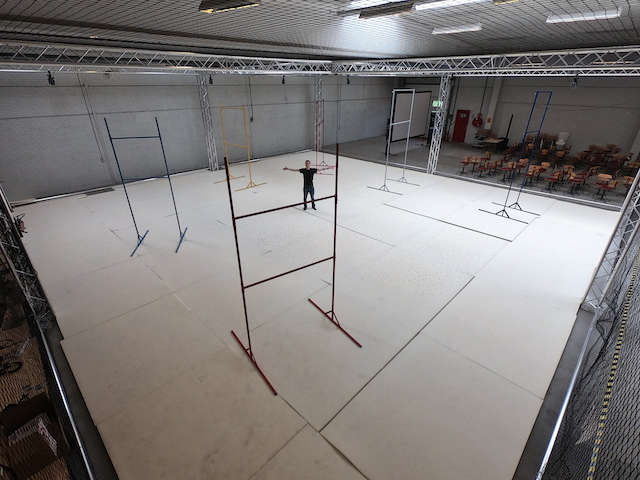
\includegraphics[width=0.5\textwidth]{figure/tiny_me.jpg}
	\caption[Custom-built obstacles around the author in AiR Lab]{Custom-built
		obstacles around the author in AiR Lab, Skejby: 12 V8 Vicon cameras,
		$15 \times 15 \times 5$ meters of flight arena.}
	\label{fig:mygates}
\end{figure}

